\chapter{Капище Волоса}

    Пока мы не отправились на северо-запад вдоль Кирилловских высот и находимся близ Щекавицы и Подола, попытаемся выяснить, где в старину находилось капище Волоса, скотьего бога. Это обсуждение пригодится и много позже, но – не буду раскрывать все карты сразу.

    Глава эта получилась из переработанного сценария второй серии моего видеоцикла про язычество Славян, которая в свою очередь заимствовала материалы из «Ереси», таким образом получилась отдача.

    Где в Киеве стояло капище языческого бога Волоса? Какие христианские святые приобрели в представлениях народа свойства Волоса как покровителя домашних животных?

   «Скотий бог Волос» – так он проходит в давних письменных источниках. Очень сложно рассуждать о языческих богах на основе летописей, житий и поучений, когда упоминаются в лучшем случае только имена. Вот Грекам повезло. В литературных памятниках четко расписано, что Гефест – хромой бог-кузнец, Гера – жена Зевса, Афина – богиня войны, Афродита – красоты, и так далее, кто кому родич, враг и друг.

Попробуем восстановить всё, что можно, о Волосе. Нам помогут письменные источники и... христианские святые – ведь славянское православие впитало в себя языческие верования, а почитание определенных богов заменилось на почитание некоторых святых. Так, Илья-пророк сопоставляется с Перуном, а святой Власий – со скотьим богом Волосом, поэтому связанные с последним обряды, сохранившиеся в народе, можно полагать применяемыми во время стародавние к Волосу, учитывая, конечно, что обряды с течением лет могли измениться.

Еще – употребляю имя Волос, а не Велес, ибо в источниках, которые я использую, всюду именно Волос.

Илья-пророк. Церковь в его честь стояла в Киеве еще до летописного крещения Руси Владимиром. В Повести временных лет за 945 год по официальной хронологии сообщается о мирном договоре между князем Игорем и Греками, то бишь Византией. Договор заключался, можно сказать, перед богами. Это с тех пор еще сохранилась присказка «бог мне свидетель».

Существовал обычай «ходить роте»  –  клясться при заключении договора. Вот как описывает Ипатьевский список Повести временных лет подобную клятву – князь Игорь с греческими послами водит их и свою дружину к определенным местам в Киеве, где приносится клятва.

\begin{quotation}
и наутрея призва Игорь сли и приде на холъмы кде стояше Перун . и покладоша оружья своя и щиты . и золото . и ходи Игорь роте . и мужи его . и елико поганыя Руси
\end{quotation} 

Утром Игорь призвал византийских послов и повел их на некие холмы, где стоял Перун. Неизвестно, та ли это гора, где через 35 лет поставит идолов князь Владимир, или другая. И вот Игорь и поганая – языческая часть народа Русь, дружина, бывшая с Игорем, закрепили там договор, положив оружие свое, щиты и золото. 

Летопись продолжает:

\begin{quotation}
а хрстьяную Русь водиша в црквь стго Ильи . яже есть над руцьемъ  конець Пасыньче  беседы . и Козаре . се бо бе сборная цркви . мнози бо беша Варязи хрстьяни
\end{quotation} 

А христианскую часть Руси Игорь повел приносить клятву в церковь святого Ильи, что над ручьем в конце Пасынче беседы и урочища Козаре. Это была соборная церковь, поясняет летописец, ибо многие Варяги были христианами. Не буду сейчас рассуждать, где находилась церковь и урочище.

Однако уточню – заключается договор между Игорем и его людьми – дружиной, приближенными – которые принадлежали к славянскому народу Русь и были варягами. Эта Русь держалась в Киеве в то время несколько обособленно от местного населения, других Славян – народа под названием Поляне. Позже Русь растворилась, смешавшись, в Полянах так же, как растворилась в других подчиненных ею землях от Новгорода до Киева и ниже по Днепру.

Итак, Игорь привел послов на холмы, где стоял Перун. Бог Волос не упомянут. Упомянут он в летописи ранее, в 907 году по официальной хронологии, когда Вещий Олег в Царьграде тоже заключал мирный договор с Греками. При этом, в Царьграде происходит вот что – Греки клянутся, целуя крест,

\begin{quotation}
а Ольга водиша и мужии его на роту . по Рускому закону . кляшася оружьемь своим . и Перуном богом своим . и Волосом скотьим бгом . и оутвердиша мир
\end{quotation}

Итак, Ольга и его людей водят куда-то на роту, по «рускому закону», где они клянутся оружием, Перуном богом своим, и Волосом скотьим богом.

А почему, в повествовании, от Русов отделена принадлежность Волоса? Смотрите – «Перуном богом своим», то есть Перун это бог Русов, свой для них бог. И отдельно указано «и Волосом скотьим богом». Русы \textbf{клянутся} им, но не сказано, что он \textbf{их}, сказано – \textbf{скотий} бог.

Однако в другом месте летописи прямо указано, что народ Русь верует в скотьего бога Волоса. Вот князь Святослав клянется в договоре:

\begin{quotation}
веруем в Перуна . и в Волоса бога скотья
\end{quotation}

Снова – Перун просто Перун, а Волос – «скотий бог», так, судя по летописи, записывается в самом договоре. Почему не указано, скажем, громовержец Перун и Волос скотий бог? Но Перун просто Перун, однако Волос везде, где упомянут в летописи, упомянут в прибавлением – скотий бог.

Мы привыкли трактовать это как бог-покровитель животных, домашнего скота. Но слово скот и производные имело и другие значения. Например, есть слово «ск\'ота» – пещера.

В летописях и других источниках на старославянском слово «скот» употребляется следующим образом. Например, в пересказе Библии в той же Повести временных лет перечисляется: «звери и скоты и гады земныя». То есть можно предположить, что скот – это домашние животные, а звери – дикие.

Там же в пересказе Библии есть разделение:

\begin{quotation}
и живяху стотьскы человецы, и бе Ной един правденен в роде сем.
\end{quotation}

То есть люди жили по-скотски, один Ной был праведен в этом роде.

Но в летописях и в давнем сборнике законов Правде Роськой слово «скот» употребляется также и в другом значении – некой суммы денег. Напомню, как Ярослав Мудрый, делает с новгородцев побор, чтобы нанять Варягов:

\begin{quotation}
и начаша скот брати от мужа по 4 куны,
а от старосте по 10 гривен, а от бояр по 70
гривен; приведоша Варягы, и вьдаша им скот, и совькупи Ярослав воя многи.
\end{quotation}

Отмечу, что слово «скот» в значении денег или какого-либо ценного, передаваемого имущества постепенно вытеснилось из письменных источников, его заменили различные именования денег и слово «товар».

Исследуя вопрос скотьего бога Волоса, мы должны рассматривать все варианты значения слова «скот», чтобы получить возможность истолковать значение, свойства этого бога.

Почему я зацепился за всё это, не проще ли считать, что скотий бог означает покровитель домашнего скота?

Но если языческие боги имели свои области покровительства, то, например, логично было при заключении определенных договоров скреплять их клятвой перед теми богами, к которым эти договоры относятся. Например, применительно к языческой Греции – торговый договор заключать перед богом торговли Гермесом.

Договоры между Русью и Византией можно считать военно-экономическими. Допустим, Перун – бог воинственный. Но при чем тут скотий бог Волос как покровитель 
домашнего скота?

Само имя Волос на славянских языках говорящее. Волос, волосы. Может, это имя-прозвище, и Волоса считали волосатым?

А какие еще слова похожи на «волос»? Поразмышляем. Вол – бык, тур. Близко к теме покровителя скота.

Есть еще слово «волость». Волость в старину это, как бы сейчас сказали, административно-территориальная единица. Слово «волость» означало также власть. Откроем словарь Даля: «стар. власть, правительственная сила». Это от «володарь», «володети». Корень тут в слове «воля», означающем приказывающее желание, власть. Царь объявил свою волю. На всё воля божья.

Если Волос – бог власти, воли, то понятно его соседство с Перуном при заключении межгосударственных договоров. Но если Волос – бог власти, то почему скотий?

Как увидим далее по сохранившимся обрядам, народ связывал Волоса именно с домашним скотом. И тому есть дополнительные доводы в топонимике Киева, хотя не всё здесь однозначно.

Расхожее мнение состоит в следующем – в Киеве на Подоле есть улица Волошская, а около нее церковь Введения, поставленная на месте более давней церкви святого Власа, который-де заместил собой в народных представлениях бога Волоса, и что на месте этой стародавней церкви и было капище Волоса.

Корни этого мнения покоятся в книге 1820 года Максима Берлинского «Краткое описание Киева», где прилагается карта и к ней описание. На странице 192 читаем:

\begin{quotation}
Капище Волосово\newline

На плане под номером 114 значится деревянная в Киево-Подоле приходская церковь Введения Пресвятыя Богородицы.
По находящейся в Киево-магистратском архиве одной выписке 1696 года, которая, судя по слогу, должна быть переписана с древней какой записи, видно, что в том месте существовало капище или божница идола Волоса, и что со времени просияния христианской веры построена там церковь Св.Власия, по сходству прежнего имени (как и теперь простолюдины в России к сему святителю прибегают для помощи в скотоводстве).

Улица, мимо церкви проходящая, называлась Быдлогонную, от польского слово быдло, рогатый скот, по тому, что тем путем к Волосовому кумиру для мнимаго пользования скот пригоняли.

По изстреблении в 1651 году во время военное Власиевской церкви, настоящая Введенская в 1718 построена. Близость скотопасного луга (оболони) может быть причиною, что сия божница устроена была так далеко от города.
\end{quotation}

Конечно, хочется верить Берлинскому и документу 1696 года, на который он ссылается.  

Лаврентий Похилевич в книге «Монастыри и церкви Киева» 1865 года пишет про ту же Введенскую церковь:

\begin{quotation}
Введенская деревянная в Плосской, или низменной части Киево-Подола, называемой Оболоньем по преимуществу населенном рыболовами. В этой части ныне находится между прочим и рыбный рынок.

По истреблении пожаром в 1651 году первой известной церкви, построенной, по мнению некоторых, на месте бывшего капища скотского бога Волоса, во имя св. Власия, настоящая Введенская церковь построена в 1718 цехмистром рыбальского цеху Павлом Демьяновичем Лесницким. Ныне она довольно обветшала; почему прихожанами взят план на построение новой каменной церкви, с приделом св. Власия, которого часть св. мощей хранится в олтаре.

К сожалению место для новой церкви избрано другое, ближайшее к центру Киево-Подола и в конце прихода, а нынешнее историческое место оставляется. Разлив Днепра почти ежегодно заливает большую часть Введенского прихода; а в 1845 году, когда высота весенних вод достигала самых высших пределов, разлив покрывал поверхность земли вокруг Введенской церкви на полтора аршина. Оттого эта часть города принадлежит к беднейшим.
\end{quotation}

Что же, не самое удобное место для капища одного из основных богов – заливаемая часть Подола, вернее даже «Плосской» слободы, но быть может, в великокняжеское время дело с паводками обстояло иначе.

Кстати, Плоская слобода, она же в народе Плоское – не искаженное ли это «Влоское», «Влошское», «Волошское»? Попробуйте произнести Плоское с полным ртом... Звуки «п», «б», «ф», «в» очень легко взаимозаменяются.

Похилевич пишет, что новую Введенскую церковь собирались строить на другом месте.

Однако, сверяясь с планом Киева 1803 года,
нынешняя Введенская церковь, что имеет адрес Почайнинская 27/44 и находится на углу с улицей Ярославской, построена примерно на том же месте, где была разобранная в 1936 уже каменная, то бишь кирпичная Введенская, возведенная в 1882-85 годах рядом с упомянутой Похилевичем деревянной. А значит, ни о каком новом месте речь не идет, 
преемственность положения сохранилась.

Современная сетка улиц Подола возникла после большого пожара 1811 года\footnote{Живший в Петербурге шотландец Уильям Гесте в 1812 году разработал план послепожарного, и так сказать, прямоугольного Подола. Считается, что его разработал главный архитектор Киева Андрей Меленский, на деле же вышло иначе. Меленский в своем проекте 1811 года, года большого пожара, сохранил устоявшуюся за столетия структуру Подола. Но его план не утвердили, а Гесте, ознакомившись с планом Меленского, создал свой план, не учитывая рельефа местности. Не сильно посчитался Гесте и с существующей сеткой улиц – фактически, была создана новая, на прежних местах остались считанные улицы. Так что Меленский, отстраивая Подол, воплотил в жизнь план Гесте. А вот свои планы Меленский воплощал, например, в нижнем памятнике Владимиру – более известном ныне как колонна магдебургскому праву, также в церкви-ротонде на Аскольдовой могиле, Крестовоздвиженской церкви на углу Гончаров и Кожемяк... По проекту Меленского построены и церкви Николы Доброго, и Рождества Христова на Подоле, где отпевали Шевченко, и многое другое. Да и Крещатик был распланирован именно Меленским. Могила архитектора сгинула вместе с кладбищем на Щекавице...}. До него улицы были кривые, застройка хаотичная. Прежняя Введенская улица шла совершенно иначе, нежели современная, которая не примыкает к церкви.

Тот, допожарный Подол, имел несколько как бы основных узлов, и северным был нынешний перекресток улиц Нижнего и Верхнего Вала с Волошской улицей, которую после 1811 года тоже проложили иначе. 

До пожара, в северном узле соединялось еще больше улиц, а через заключенную в канал речку Глыбочицу был перекинут мосток. И тогдашняя Волошская улица начиналась близ Кирилловских высот, выруливая от перекрестка у Иорданских рогаток, там где ныне перекресток Кирилловской, Нижнеюрковской и Юрковской.

На западном его углу, до устроения там кирпичных заводов, была гора – при добыче глины бо\'льшую часть ее съели. Эта гора сейчас называется Юрковицей, а прежде именовалась Лысой. Об этом мы поговорим подробно в части про Кирилловские высоты. Как вы помните, на этой современной Юрковице я предполагаю первоначальный град Киев, ту крепость, что заложили братья Кий, Хорив и Щек – вдобавок к уже существовавшим укреплениям города, который, получается, имел тогда другое название.

Итак, современная Волошская улица совсем не то, что допожарная. Волосская улица по 1811 год лежала от дома по Оболонская, 7\footnote{50°28'11.9"N 30°30'18.7"E} до Нижний Вал, 29\footnote{50°28'09.3"N 30°30'56.6"E}, или, если угодно, примерно до перекрестка современной Волошской и Нижнего Вала.

В каком-то очень далеком прошлом это был, вероятно, кратчайший путь с населенной тогда Лысой горы с ее крепостью к Подолу. Это как дорога от дворца президента, скажем так...

Конечно, при соединении такой дороги с посадом мог стоять идол Волоса, на эдакой нейтральной территории, между народом и правительством. Улица Волошская (на тогдашних картах Волоская) начала 19 века немного не дотягивала до нынешней Введенской церкви, где предполагают бывшее капище Волоса, но кто знает, как всё выглядело в веке девятом?

Однако, как я предположу далее, капище Волоса появилось в тех местах позже, и, как ни странно это звучит, после крещения Руси. Но об этом позже!

Близ начала прежней Волошской тоже было некое древнее кирпичное строение\footnote{Место его раскопок на 2022 год находтися по координатам
50°28'13.3"N 30°30'12.2"E – это за домом непосредственно на север от упомянутого перекрестка Кирилловской и Нижнеюрковской – со стороны улицы Юрковской, по третьему номеру там стоит деревянная церковь, ибо в раскапываемых уже много лет развалинах археологи предполагают церковь 12 века.}. 

А мы снова вернемся к Введенской церкви и ее связи с более ранней церковью святого Власа. Последняя сгорела во время пожара в 1651 году. Введенская же построена в 1718-м. 67 лет разницы. Мне кажется сомнительным, чтобы на тогдашнем тесно и хаотично застроенном Подоле место оставалось пустым почти 70 лет. 

Как бы ни было, положим, Введенскую построили на месте церкви святого Власа. А связь \textbf{ее} места со святилищем бога Волоса зиждется на шатком основании слов краеведа Максима Берлинского, который-де читал некую выписку 1696, вроде бы переписанную с еще более давней записи. При этом – ни одной цитаты. Я не могу принимать это за надежное основание для рассуждений.

Если мы посмотрим на перекресток допожарного Подола, по карте 1803 года, то увидим следующее. От Кирилловских высот идет улица Волоская (синяя латинская H), вот мимо Введенской, а положим бывшей Власовской церкви (красная большая М) идет от Плосского улица Введенская, прежде Быдлогонная. Между ними латинской буквой маленькая «L» обозначена Воловня – согласно Далю, «сарай, навес, крытое помещение для волов».

\begin{center}
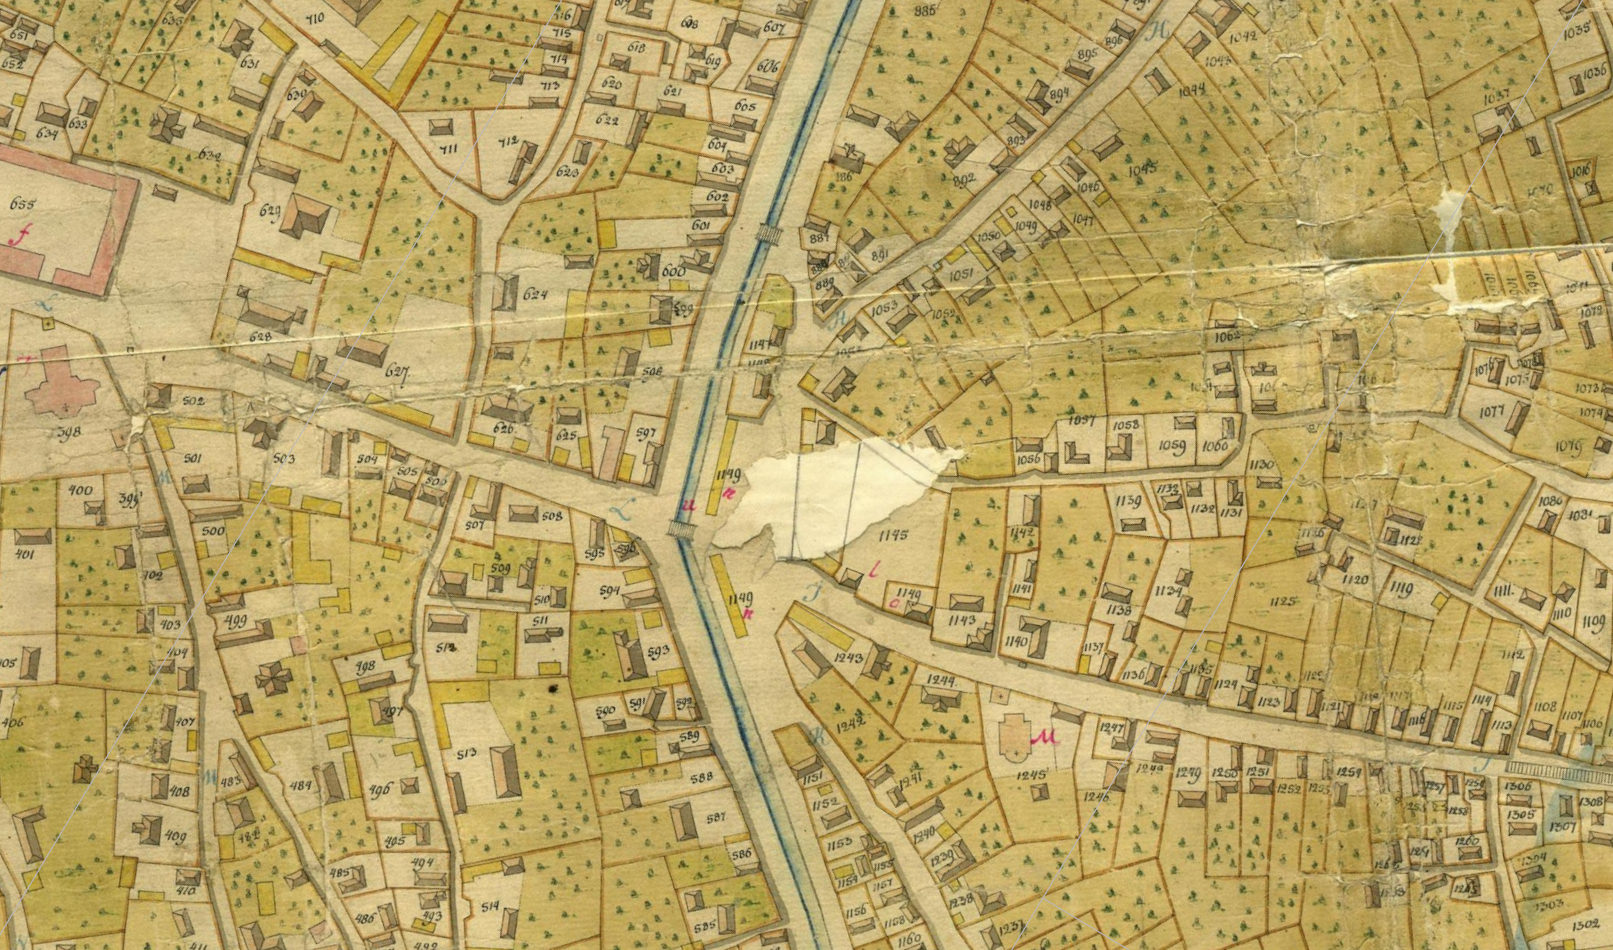
\includegraphics[width=\linewidth]{chast-colebanie-osnov/tur/volos-map-01.jpg}
\end{center}

   И вот этот вол – домашний скот, и скотий бог Волос – может они как-то связаны через корневое слово? Что вообще значит слово «вол», от чего оно произошло? Я не знаю. Может быть, вол – тот, кого ведут. Вели волов на выгон.

   Вообще говоря, волами называют кастрированных быков. А есть еще тур – туром сейчас именуют дикого быка. Слово «тур» употреблялось Славянами, князь Владимир Мономах писал о турах в поучении сыновьям. Со словом «тур» созвучно и греческое таур – бык.

Есть еще такой, примерно 17 века, неразборчиво написанный Пискаревский сборник со статьей, что начинается примечанием «Выписано из книг летописца о идолех владимировых», с перечнем идолов, которых поставил князь Владимир в Киеве. И к известному традиционному списку добавлены: «Волос, Позвизд или Похвист, Ладо, Купало, Коляда», а еще говорится о Леле, Полеле и Туре-сатане. Вероятно, составитель рукописи тащил в нее сведения из разных источников, не задумываясь об исторической правда, и о том, что разные имена могут относиться к одному и тому же божеству. 

   Про Тура сказано:
 
\begin{quotation}
\noindent Начелше от самого рожества христива на святые дни собирающегося на богомерзкие игрища, песни поют, и в них аще и о рожестве христове вотпоминаю, но зде же беззаконно и коляду ветхую прелесть диавольскую много потворяюще присовокупляют к сему на тых же своих законопротивных соборищах и некоего Тура сатану и протчие богомерския скареды воспоминают
\end{quotation}


   К чему это я завел разговор? Современная улица Волошская пересекается с улицей Туровской. Корни ее названия уходят в такое же глубокое и темное прошлое, как и допожарной Волошской.

   В северной части Подола было урочище Турово. Я уже писал про связанный с урочищем водоём Турец, или, в более давних земельных документах, смуговина Турец. По совокупности данных, урочище Турово находилось как раз примерно у начала допожарной улицы Волошской. Если угодно – окрестности остановки Оболонская.

   В летописях один раз упомянута Турова божница. В сообщении за 1146 год, когда Игорь Ольгович звал киевлян на гору на Ярославль двор, киевляне собрали вече у Туровой  божницы и звали князя к себе, а он послал взамен своего брата. Вот и всё.

Вопреки популярным представлениям про «вече» – мол, собирался весь честной народ и решал государственные дела – в летописях есть подробность, что собирался не весь честной народ, но конный, стало быть люди зажиточные, либо военное сословие.

   В списках Пролога 15-16 веков появляются сведения о том, что в месте крещения киевлян теперь, то есть в 15-16 веке, стоит церковь святых мучеников у Турова. Списки переписывались, церковь «у Турова» превратились в церковь святого мученика Турова, и вот уже начали придумывать, что Туром звали того варяга-христианина, чьего сына при князе Владимире решили по жребию принести в жертву, и дескать, христианское имя Тура было Феодор.

   Различные археологи помещают Турову божницу то на улицу Борисоглебскую, то в окрестности Почтовой площади, то на Контрактовую площадь – короче говоря в совсем другой стороне Подола, нежели где протекал уцелевший в топонимах ручей Турец.

   Это всё равно что дать человеку в руку банан, очистить его, предложить съесть, но человек банан выбросит, потом полезет на яблоню и, сорвав оттуда яблоко, скажет – вот банан!

   Итак, мы определили некоторую смежность положения допожарной улицы Волошской и урочища Турово. Также не может ускользнуть от внимания и общность слов тур и вол, однако, тур был диким зверем, а вол – относился к домашнему скоту, и мы знаем из летописи, что Волос – это скотий бог.

   Принято считать, что христианский святой Власий или Влас перенял на себя, в народных представлениях, свойства бога Волоса. Прежде чем мы коснемся этого подробнее, затрону тему календаря.

   Если вы откроете сборники житий святых, то обнаружите, что жития расположены по святцам – дням поминовений тех или иных святых, апостолов, или просто библейских событий. Согласно святцам раньше выбирали имена новорожденным. Существует также устный народный календарь, или месяцеслов – те же святцы с привязкой к каждому дню примет, поговорок, поверий. Нет какого-то единого месяцеслова – имея общую основу, в частностях он меняется от местности к местности, а предания и поговорки передаются из уст в уста, из поколения в поколения, эдакое распределенное между людьми знание и представления.

В месяцеслове запечатлено произошедшее некогда наложение христианства на бытовавшие языческие верования. С чьей стороны произошло это наложение? Сие важно выяснить, чтобы понять – это на день святого Власия Севастийского, 11 февраля по старому стилю народ и прежде, до христианства, выполнял обряды, связанные с Волосом... Или же напротив, до принятия христианства обряды, связанные с Волосом, отправлялись в другой день, а с принятием христианства были перенесены на 11 февраля, на день святого Власия?

    Откроем житие святого Власия... Поначалу я взял латинские, а не славянские варианты жития, чтобы исключить возможное влияние верований в скотьего бога Волоса, но затем подумал – ведь и латинские жития могли быть сложены в странах, которые прежде были населены славянами. 

   Что же говорят латинские жития?

   Власий Севастийский, врачеватель, жил в Малой Азии при императорах Диоклетиане и Ликинусе, то бишь, по официальной хронологии, на стыке 3-4 столетий нашей эры. Был епископом города Севастии в Каппадокии, ныне это турецкий город Сивас.

   Скрываясь от гонителей, Власий удалился в пещеру в горе Аргэос. К нему приходили дикие звери и ожидали, пока святой завершит свою молитву, после чего он благословлял их. Также Власий исцелял больных животных наложением рук.

   Что же, хотя и не скотий бог Волос, но имеет отношение к животным, и похож именем. Вот выжимка данных из католических источников по святому Власию – сент Блезу. День поминовения 3 февраля. Покровитель, кроме прочего – животных, а также чесания шерсти и торговли шерстью. Это кажется мне крайне любопытным. Шесть – волосы. Влас – Волос. Хотя связь Власия с чесанием шерсти обоснована в житии – Власия пытали при помощи чесалок.

\begin{center}
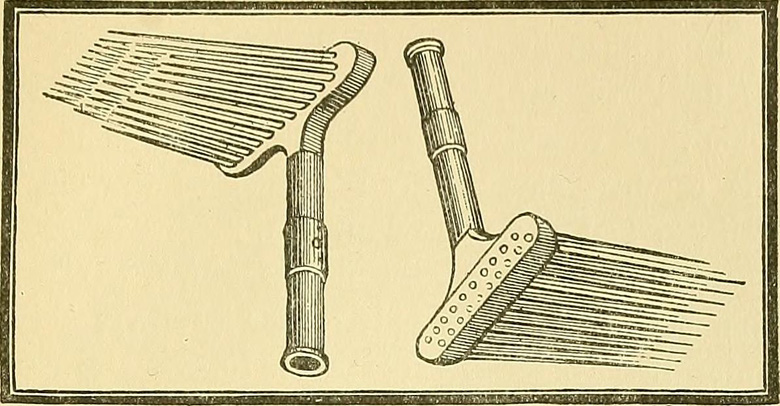
\includegraphics[width=0.50\linewidth]{chast-colebanie-osnov/tur/combs.jpg}
\end{center}

   В католическом мире Власий стал популярен в 11-12 веках, и появился своеобразный ритуал – в день поминовения этого святого, который считается также исцеляющим от болезней горла, благословлять против этих болезней при помощи двух перекрещенных свечей, как бы рогов.

   Корни источников вариантов жития святого Власия невозможно отследить. Самые ранние упоминания Власия, вероятно, приведены не в житиях, а в книгах по медицине греческого лекаря Аэция Амидийского (Ἀέτιος Ἀμιδηνός), который жил, как считается, в 5-6 веке. И дескать, Власий искусно, палочками извлекал застрявшие предметы из горла.

   Каковы же первоисточники жития Власа – неведомо. Хорошо известно, сколь различны бывают списки житий, отличаясь сюжетом и действующими лицами. Есть у житий разных святых и похожие места, написанные как под копирку, стало быть придуманные, когда сочинитель не обладал сведениями, однако должен был что-то сообщить, допустим, о рождении и юношестве святого. Таким образом многие святые действовали и умирали во времена известных гонителей христианства, а родителями героев повествования были благочестивые люди. 

   У славян было принято писать «жития», а в западном мире для этого существует другое обозначение, мартиролог, мученичество, потому что ближе к концу повествования святой проходит невредимым различные мучения, а затем ему отрубают голову. 

    Мы не можем установить, на основании каких исторических событий возникли жития святого Власа. Мы знаем лишь, что какие-то жития ходили в списках, по крайней мере с 11-12 веков.

   Давайте обратимся теперь к славянским источникам. Будем держаться подальше от книг современных ученых и Википедии, сузим наш круг чтения до того, что могли читать сельские батюшки и грамотеи, да пересказывать это другим.

   В давнем Прологе есть кратенькое житие Власия, что сей бяше во времена Ликиния царя, епископ Себлетийский. Живя в некой пещере в горе, он укрощал диких зверей и многие цельбы творяще.

   В Житиях святых святителя Димитрия Ростовского, составленных в 17 веке, в издании 19 века на февраль приходятся целых два дня поминовения Власия. Удивительно, правда? В издании 1764 года, изданном почти век спустя составления Димитрием, Власий в феврале один, за 11 число, а вот в 19 веке уже два Власия, на 3 и 11 число.

   На 3 февраля (по старому стилю, конечно) – память святаго мученика Власия, и дано примечание – он же именуется Вукол, от греческого вуколос, пастух.

   Запомним это – пастух! И Вукол тоже запомним! И конечно, сопоставим со скотьим богом...

   В житии сказано:

\begin{quotation}
Святый Власий был пастух и происходил из Кесарии Каппадокийской – дается примечание, что Каппадокия находилась на востоке Малой Азии, и Кесария – главный город Каппадокии.

   Когда наступило гонение и отыскивали христиан, то и Власия, как христианина, искали по всем окрестным местам. Узнав об этом, святый Власий добровольно отдался в руки мучителей, которые растянули и били его воловьими жилами. Но бог излечил его болезни и исцелил от ран. Узнав об этом, правитель назвал это чудо волхованием и велел после тех мучений ввергнуть святаго в котел с кипящей водой. К ужасу всех присутствующих, мученик остался невредим и в кипятке разговаривал с окружающим его народом, ибо явились ангелы божии и сохранили мученика невредимым. 
\end{quotation}

Дважды правитель посылает к пребывающему в кипятке Власию воинов, но все они, увидев чудо невредимости, обращаются в христианство. Читаем далее:

\begin{quotation}
Вслед за этим сам правитель пришел сюда и увидел святого, находящимся в кипящей воде. Думая, что вода остыла, правитель умыл лицо свое в этой воде, и тотчас обварил лицо свой, и от того умер.

   Обратив многих своими чудесами ко Христу, святый Власий помолился Богу и предам ему свою святую душу. А пастушеский жезл Власия, будучи водружен в землю, возрос в огромное дерево, которое ветвями своими покрыло алтарь церкви, созданной над мощами святого – и следует приписка: Святый мученик Власий жил и скончался в 3 веке.
\end{quotation}

Пролистаем теперь книжку до дня 11...

\begin{quotation}
Житие и страдание святаго священномученика Власия, епископа Севастийского, и других пострадавших с ним.
\end{quotation}

   Как и его тёзка-пастух, жил в Кападдокии – только в другом городе, в Севастии, где христиане выбрали Власия епископом. Происходило дело при Диоклетиане, то бишь на стыке 3-4 веков... Описывается уже ведомая нам жизнь Власия в пещере, общение со зверями и врачевание оных. Затем игемон Агриколай ужесточает гонения на христиан. Власия находят в пещере, он радостно идет с посланцами игемона, по пути совершает всяческие чудеса и врачует. Кстати, в отличие от католических представлений на этот счет, тут ничего не сказано о том, что до епископства своего Власий был врачом. 

   По пути к игемону Власий встречает некую вдову. На этом важно остановиться подробнее, а почему – вы поймете позже.

\begin{quotation}
Одна бедная вдова не имела ничего, кроме одного поросенка. Волк, подкравшись, схватил его. Бедная женщина стала горько плакать. Увидев, что идет святой, она бросилась к нему и со слезами стала рассказывать ему о своем горе. Святый, улыбнувшись, сказал ей:

 – Не предавайся скорби, женщина, не плачь, твой поросенок будет возвращен тебе живым и невредимым.

   Сказав сие, святый продолжал свой путь, а к убогой вдовице прибежал тот волк, неся в зубах ея поросенка. Он отпустил его перед нею безо всякого повреждения и убежал обратно в пустыню.
\end{quotation}

Когда же, позже, игемон заключил Власия в темницу, то вдова

\begin{quotation}
заколола своего поросенка, которая невредимым получился из зубов волка, сварила голову и ноги, положила на блюдо, сюда же она добавил еще семян, земных плодов и огородных овощей. Спрятав все это в корзинку, и зажегши свечу, она принесла эту корзинку святому в темницу. Припав к ногам мученика, стала умолять его, чтобы он взял эту пищу и вкусил ея. Воздав хвалу богу, святый вкусил принесенной пищи, затем, благословив вдову, он сказал ей:

 – Женщина, таким образом совершай каждый год мою память – тогда ничто из нужного в доме твоем не оскудеет, если же кто другой уподобится тебе и будет совершать мою память, тот получит в изобилии дары Божии и благословение господа пребудет на нем во все время его жизни.
\end{quotation}

   Понимаете, что это значит? Описан обряд заклания жертвы и приготовления обрядового блюда в определенный день, день поминовения. Святой ли Власий предписал сие, или сюжет с вдовой и закланием поросенка появился в житии, чтобы привязать существующий, бытующий обряд к повествованию о житии святого?

   Далее мы еще вспомним об этом обряде, в неожиданной связи.

   Я не буду пересказывать далее житие, скажу лишь, что Власия лишили головы – только так удалось убить его. Обезглавливание, кажется, было основным способом окончательной казни святых мучеников, ибо ничто другое им не вредило, либо вредило временно.

   В примечании к житию указано, что Власий скончался около 316 года, мощи его перенесены на Запад во время крестовых походов , части их находятся во многих странах Европы.

   Прежде чем отправляться в нашем исследовании дальше, немного передохнем и остановимся еще на датах, указанных в этих православных житиях.

   3 февраля по старому стилю – день мученика Власия из Кападокии, пастуха. Напомню – в католической церкви 3 февраля по новому стилю, то бишь по григорианскому календарю – день поминовения святого Власия.

   11 февраля по старому стилю, по юлианскому календарю, в православном житии – день опять же мученика Власия, тоже из Кападокии, но из другого города, и уже епископа.

   Примечательно, что разница между днями примерно – с погрешностью в пару дней – указывает на разницу между юлианским и григорианским календарями. Можно подумать, что редакторы Житий, уже после Димитрия Ростовского, нашли святого Власия в некоем списке католических святцев, за 3 февраля, и переписали оттуда статью про него, а в том источнике Власий был пастухом. Однако статья о святом Власии за 11 юлианское февраля более-менее соответствует иному, широко известному латинскому, католическому житию, вместе с сюжетом про вдову и поросенка. Желающих отсылаю ко главе 38-й Золотой Легенды – латинской книги житий святых 15 века.

    Житие про Власия-пастуха несомненно выписано из какого-то иного источника. Оно сжато – краткость противник выдумки, из него можно выделить главное свойство Власия – пастушество и жезл пастуха.

   Какие же народные поверья и предания связаны с Власьевым днем и с каким именно?

   Из книги первой половины 19 века Сахарова «Сказания русского народа», за 11 февраля по старому стилю указано:

\begin{quotation}
Набожные поселяне в этот день служат молебны св. мученику Власию и молят его о покровительстве и защите домашнего скота, особливо коров. Во имя его прихожане устраивали в старину приделы и часовни. Прасолы, торгующие скотом, в Зарайске и других городах, перед началом своего торга служат молебны св. Власию. 

В Вельском уезде Вологодской губернии, в Ракульском погосте находится древняя церковь, выстроенная в лесу, во имя св. Власия. Сюда съезжаются поселяне для молитвы св. угоднику. Поселянки приносят в храм коровье масло и кладут его пред образом св. угодника. Это масло называется в Вельском, Череповецком и Белозерском уездах «воложным». 

В Шенкурском уезде молебствие совершается в субботу перед Пятидесятницею. Тогда к церквам приводят коров для окропления св. водою. То же самое отправляют и во время скотского падежа.
\end{quotation}

   Волосовские, или Власьевские морозы считались последними, и ходила поговорка – Власий сшиба роги с зимы.

   На Харьковщине в старину был обычай, когда женщины ходили в этот день в шинок пить водку – чтобы коровы были ласковыми. Вернувшись домой, они обрядово били мужей так называемыми донцами, чтобы были послушными. Донце – это часть составной прялки для льна, ее подставка.

%5da86acade821a50313bc810-middle.jpg

   Другой частью такой прялки является гребень, вставляемый перпендикулярно в донце. Именно гребнями, впрочем допустим в Англии считали, что для чесания шерсти, а не льна, мучали, согласно житию, святого Власия.

   По всей Украине на Власа ходили с иконой и святой водой в стойла и освящали скот.

   Что же, Власьевский день, 11 февраля по старому стилю, 24 по новому – богат на обряды, связанные с домашним скотом, и находим обряд с отголоском в связи с пряжей. Но ведь славянское слово «волос» тоже связано с прядением. Волос это не только волосы как шерсть. Волос это еще и нить.

   Как бы ни было, с Волосом мы имеем на уровне языка прямую смысловую связь с волами и волосами.

   А что насчет греческого имени?

   Греческое имя Βλάσιος, присущее святому, на греческом ничего не означает, как бы разные толкователи ни пытались вывести его из других греческих слов. Это заимствование. Некоторые ученые думают, что Βλάσιος – искаженное греческое βασιλεύς – царь, император.

 Латинизированный вариант Власия –  Blasius производят от латинского blaesus – шепелявый.

   Мы натолкнулись на любопытную штуку. Вот святой, который, согласно житию, жил в грекоязычной Каппадокии и должен был иметь греческое имя. Однако его имя вовсе не греческое, оно огреченное. Корень этого имени – Влас, а дальше добавлено греческое «иос». Власиос.

   То есть, Власиос – это огреченный славянский Влас или Волос, потому что в славянском языке волос и влас это одно и то же. Почему у описанного в житиях святого, который был, упрощенно говоря, греком по языку, а обитал в провинции Римской империи Каппадокии, славянское имя на греческий лад? Имя, которое соответствует имени славянского скотьего бога? Почему этот святой связан с покровительством животным и прядением, так же, как скотий бог?

   Вопрос о первичности решается очень просто – если на одном языке можно понять смысл, а на другом нельзя, значит первичность слова относится к первому языку.

   Возьмем латинское «futurum» или английское «future». Будущее. Языковеды расскажут вам о каких-то праиндоевропейских корнях. Вообще вот это размытое словосочетание – индоевропейский... Кто испокон веков жил от Индии до Европы? Славяне. Но ученым угоднее  размыто уходить от прямоты и говорить – индоевропейский, или еще туманнее – праиндоевропейский.

   Ладно. Английское «future» произносится не так, как пишется, а давайте произнесем как пишется:\newline

FUTURE\newline

ФУТУРЕ\newline

   Некоторые звуки легко меняются при выговоре. Например, стоит глуше произнести «д» – Дмитрий, и получится «т» – Тимофей. А скажите плотнее звук «ф» и выйдет «б».

Произнесем теперь ФУТУРЕ, применив этот иной выговор.\newline

БУДУРЕ\newline

Ага, у англичан БУДУре – а у нас БУДУщее. В русском языке, а не каком-то праиндоевропейском, мы нашли общий корень – буду. И это не заимствование, ибо имеет смысл в связи со смежными словами – быть, буду, был.

Есть ли для слова future такие значащие корни в английском языке? Нет. Есть ли в латыни для futurum? Тоже нет, иначе ученые не прибегали бы к высасыванию из пальца выдуманных ими пра-индо-европейских слов.

   Так что думать про святого Власия, Власиоса – малоазиатского христианского святого с огреченным именем языческого славянского бога?

    Но только ли один святой Влас перенял на себя свойства скотьего бога Волоса? Прежде чем развивать эти соображения, коснусь важного вопроса – какой календарь использовали славяне до принятия христианства? После принятия, спустя некоторое время – юлианский, а затем уже при Советском Союзе – Григорианский. А вот \textbf{до} христианства? 

   Как считали дни, недели, месяцы, годы? Был ли этот счет единым, по всем землям, которые Нестор летописец именовал Великая Скуфь? 

   Допустим, две тысячи лет назад... Я живу в лесу на глухом хуторе, в какой-нибудь избушке или глинобитной хате. Вот я просыпаюсь утром – ага, начался новый день. Но у меня нет компа, нет наручных часов, нет бумажного отрывного календаря. Как мне считать дни? Ну, делать топором зарубки на каком-то бревне. 365 зарубок нанес – год прошел, беру другое бревно.

   А откуда я знаю, что год это именно 365 дней? Да, у нас есть сведения, что люди в те давние времена как-то считали дни и годы, платили в определенное время дань, наконец – \textbf{праздновали} в определенные дни. Значит, неким образом была развита астрономия, и наблюдение за небесными телами – этим звездным хронометром – позволяло вести учет времени на земле. Для развития астрономии нужны многолетние наблюдения и возможность записи и сохранения этих наблюдений, а также передача записей и способа наблюдений другим людям в других местностях.

   Чтобы год стал годом – чтобы знать, сколько дней в году – то есть время, за которое Земля совершает полное обращение вокруг солнца – нужна развитая астрономия. 

   Представление о годе является условием для периодического отправления обрядов и праздников. Нам нужно знать, что 3-го или 11-го февраля, или такого-то по счету месяца, мы празднуем святого Власа или скотьего бога Волоса.

   Но можно пойти другим путем, создать календарь на более простом уровне, и вероятно до \textbf{развития} астрономии люди поступали именно так.

   Самое простое это считать дни. Считать дни можно даже на необитаемом острове.

   Но дни нужно как-то упорядочивать. Так появляется понятие недели. Замечу – многие народные празднования отмечаются целую неделю. Масляная неделя, Русальная и так далее.

Мы привыкли к тому, что неделя состоит из 7 дней. Корни такого представления лежат в Ветхом Завете Библии – шесть дней бог творил землю, а на седьмой отдохнул. Этот седьмой день в иудаизме – шаббат, суббота. Неделя у иудеев, также как например в США, Англии и Канаде, начинается с того дня, что мы называем воскресеньем. 

Первый день недели в США это sunday – наше воскресенье, а выходные там суббота и воскресенье, то есть первый и последний дни их недели.

У нас в неделе выходные выпадают на те же дни, но началом недели считается понедельник.

Как видим, понятие недели – условно, и складывается кроме прочего по религиозным соображениям.

Какой же неделей пользовались славяне до принятия христианства?

Хотя в старославянском языке есть слово седьмица, указывающее на седьмой день недели, слово это относится уже к христианскому времени. Иудейскую субботу те славяне, которые не исповедовали иудаизм, не чтили. Если мы исключим из дней недели субботу, у нас останутся только славянские названия дней недели, на русском это:\newline

\noindent понедельник, то есть день по неделе, после недели\newline
вторник\newline
среда – буквально середина надели\newline
четверг\newline
пятница\newline
воскресенье\newline

   Но какая же среда середина недели? Серединой она была бы при пяти днях в неделе. Воскресенье так называется потому, что согласно Новому завету, в этот день недели воскрес Иисус. То есть день, следующий за субботой, в иудейской семидневной неделе, стали называть воскресеньем.

В украинском языке воскресенье обозначается словом «неділя». Ничего не делать. Запрет на действие, как в случае с иудейской субботой.

   Такой же запрет, но с ограничением определенных работ, был закреплен в народных верованиях с пятницей, иначе же следовала кара от очень интересного существа – святой Пятницы, или, как ее еще называли, русалки Пятницы.

Однако были сходные предания и о святой Неделе. А если предположить, что святая Пятница и святая Неделя – одно и тоже? Мы же видели, как в житиях святых один святой Влас разделился на двух, чтобы соответствовать двум разным дням. Почему то же не могло случиться с выходным днем у язычников-славян при переходе на семидневную неделю?

Отнимем от недели еще один день. Остается пять:\newline 

\noindent Понедельник\newline
Вторник\newline
Среда\newline
Четверг\newline
Пятница = Неделя\newline

Среда становится точно серединой недели, что соответствует именованию – Среда, Середа, Середина. А почему пять дней? Во-первых, так удобно считать, по количеству пальцев на руке. Ни семь, ни шесть дней не столь удобны, если вы живете в глинобитной хате и считаете на пальцах. Я говорю сейчас о времени зарождении календарного цикла.

   Перейдем теперь к понятию месяца. Месяц – старое название Луны. Использование слова «месяц» для обозначения определенного количества дней указывает, что это использование возникло во время, когда в ходу был лунный календарь. Ведь именно примерно за привычный нам календарный месяц Луна, она же в народе Месяц, проходит на небосводе все свои фазы.

   Это древнейший календарь. Мусульмане до сих пор пользуются лунным календарем для вычисления дат своих праздников. Лунный календарь был у шумеров, китайцев – повторюсь, это был первый календарь человечества, затем сменившийся на солнечный.

   Итак, люди видели новолуние, новый месяц и понимали – начался новый месяц в прямом и переносном смысле. В таком месяце умещалось 6 недель – 6 раз по 5 дней.

   Легко и относительно легко выявляемые астрономические явления – фазы луны-месяца, равноденствие и солнцестояние –  составили основу древнего календаря и одновременно основу для повторения обрядов из года в год в одни и те же дни, а точнее недели или на протяжении месяца.

   К этому присоединилась, вероятно, периодичность проявления, в наблюдаемой нами части действительности, существ из другой ее части, с иным течением времени – будь то умершие люди или обожествляемые сущности, взаимодействие с которыми, предполагаю, облегчено и упрощено только в определенные дни года.

   Поэтому, повторю мысль – основные празднования у язычников приурочивались не к определенному дню, а были растянуты на недели.

   Давайте снова заглянем в жития святых и народный календарь. Вот у нас есть 3-е февраля по старому стилю. Пастух Влас, оставшийся, кажется, только на бумаге. 11 февраля по старому стилю чтили покровителя домашнего скота – святого Власа. А шестого февраля по старому, или 19 по новому стилю, был праздник Вукола.

   Вукол в переводе с греческого значит пастух. Согласно житиям, Вукол жил во втором веке и был положен в епископы города Смирны то ли апостолом Павлом, то ли Иоанном Богословом. Смирна это Малая Азия, нынешний Турецкий город Измир, а раньше греческий город. Кажется, бо\'льшая половина христианских святых родом из тех краев.

   И вот этот Вукол, сведения о коем противоречивы и кратки, у славян прослыл как Вукол Телятник. Праздник его называли просто Вуколы, и считалось, что с этого дня коровы начинают телиться. Родившихся в это время телят называли жуколами. Хлев окуривали чабрецом, а коровам на Вукол давали особо много корма.

   Что же, почти подряд три праздника, связанных с домашним скотом. Случайность или закономерность? А давайте поищем еще по соседству.

   Ага, вот – день Онисима-овчарника или Овчара, 15 февраля по старому стилю, 28 по новому. Он же день под названием Овчарницы. Считалось, что святой Влас сшибает с зимы первый рог, а Овчарницы второй. Стало быть, зима представлялась рогатой. В этот день пастухи-овчары, после молитвы святому Власию – не Онисиму – окликали звезды, обрядово обращались к ним, чтобы у хозяина овец рождалось их побольше. В этот день также выставляли на утренний мороз пряжу, что называлось \textit{ зарнить}.

   Полагаю, что дни и святого Власв, и Вукола, и Онисима-Овчарника – некогда были приурочены скотьему богу Волосу, лежали в пределах отведенного ему а хоть бы и месяца. И в пользу этого есть еще доводы.

   Вернемся ко крещению киевлян князем Владимиром. В известных нам списках летописей \textbf{не} сказано, что Владимир, среди прочих идолов, низвергал Волоса.

   А вот в церковном сочинении «Память и похвала князю рускому Володимеру» по списку 16 века однако писано:

\begin{quotation}
А сам в Киев вшед, повеле испроврещи и избита кумиры, овыи иссещи, а иныя ижжещи; а Волоса идола, егоже именоваху скотья бога, веле в Почайну реку въврещи; Перуна же повеле привязати к коневи, к хвосту\footnote{Значит, идол Перуна был небольшим.} и влещи с горы по Боричеву на ручей; а слугы пристави бита идолы жезлием.
\end{quotation}

   Нет подробностей, откуда и как низвергали идола Волоса – я предполагаю, что оттуда же и точно так же, как Перуна, но об этом позже. Сказано также, что обоих идолов жезлами били «слугы».

   Что происходит, уже согласно Повести временных лет, после низвержения идолов и крещения? Владимир 

\begin{quotation}
повеле рубити црькви и поставляти по местомъ. идеже стояше кумиры и постави црквь стго Василья на холме . идеже стояше кумири . Перунъ и прочии идеже требы творяху князь и людье
\end{quotation}

Итак, Владимир повелел рубить – то есть делать из дерева – церкви, где стояли кумиры. И поставил церковь святого Василия на холме, где стояли кумиры Перуна и прочих и где им творили требы князь и люди.

   В списках летописей не упомянуты названия каких-либо других церквей, кроме Васильевской, в числе сооруженных после крещения. Вы можете прочитать в разных современных статьях и книгах сведения, что церковь святого Власия, та, на Подоле, была поставлена сразу после крещения, однако это домысел. Давние источники об этом молчат.

   Почему же Владимир поставил церковь именно святого Василия именно на холме, где стояли идолы языческих богов?

   Я полагаю, вы уже насторожились, почуяв сходство имен Василия и Волоса...

   Василий было христианское имя, принятое Владимиром при крещении. Церковь же соорудили, получается, сразу в честь князя Владимира-Василия, и в честь одного из наиболее почитаемых христианских святых – Василия Великого, из уже известного вам города Кесарии в Каппадокии. Жил в 4 веке нашей эры.

   В народе с ним было связано два праздника – Васильев вечер (вечер 31 декабря по старому стилю), и сам Васильев день (1 января по старому стилю). Нынешний Старый Новый год!

   Васильев вечер, иначе Щедрый вечер, он же Меланка – день святой Мелании. На Щедрый вечер щедровали – ходили по домам, пели песни-щедривки, а хозяев угощали щедровальщиков.

К щедрованию добавлялся обряд вожения Козы – человек цеплял себе рога, хвост, надевал шерстью наружу кожух и ходил с песенниками. К Козе иногда присоединялся ряженый в Кота.

В некоторых местностях Щедрый вечер назывался Авсень или Усень, а песенки, с которыми ходили по домам, призывая Авсень – авсеньками. Иногда в них проскальзывало слово «Коляда», и повторялось – Авсень-Коляда, хотя колядуют обычно под Рождество, а не под Щедрый вечер. 

Под Воронежом, в начале 20 века, в селе Хохол-Тростянка Острогожского района, записана весьма показательная авсенька, где охватывается большой временной промежуток, вероятно в который пелись такие авсеньки, а также скотоводческая направленность Авсеня – Авсень выступает настоящим скотьим богом:

\newpage

\textit{\noindent 
Ой, Авсеня, кочеты кричали,\newline 
Ой, Авсеня, ковали вставали,\newline 
Ой, Авсеня, топоры точили,\newline 
Ой, Авсеня, дубья валили,\newline 
Ой, Авсеня, доски пилили,\newline 
Ой, Авсеня, мосты мостили.\newline 
Ой, Авсеня, как по этих мостах,\newline 
Ой, Авсеня, три братца шло:\newline 
Ой, Авсеня, Рождество Христово, \newline
Ой, Авсеня, Василий да царевский, \newline
Ой, Авсеня, Иван Креститель. \newline
Ой, Авсеня, первый братец\newline
Ой, Авсеня, гоня лошадок \newline
Ой, Авсеня, с жеребяточками.\newline 
Ой, Авсеня, другой братец \newline
Ой, Авсеня, гоня корову \newline
Ой, Авсеня, и с телятами. \newline
Ой, Авсеня, третий братец \newline
Ой, Авсеня, гоня овечек \newline
Ой, Авсеня, и с ягненочками. \newline
Коли будете дарить, \newline
Тады будем хвалить. \newline
Не подарите вы нас, \newline
И не похвалим вас.\newline}

   Что означает имя Авсень, он же Усень? Ученые предполагают что угодно – и что это искаженное слово Осанна, и ищут корни в санскрите. Кажется, всё намного проще. Помните описание идолов у Нестора Летописца? Волос там впрочем не упомянут, зато есть описание Перуна деревяна, а голова его серебяна, а ус золот.

   Скорее всего, Волос тоже был усат – и не только, но еще и бородат. Снегирев в книге 1837 года «Русские простонародные праздники и суеверные обряды» пишет:

\begin{quotation}
В южной России, по свидетельству протоиереря Сабинина, старухи «завивали бороду Волосу» пред жатвою – собрав горсть колосьев и не вырывая их из корня, перегибали и завивали в узел, в знак того, чтобы до них не касалась рука жницы.
\end{quotation}

   Где борода, там и усы. Так вот имя или прозвище Усень – чисто славянское, оно означает Усатый. Усень! В украинском есть сходное слово – «вусань», то бишь усач. Такие слова, заканчивающиеся на «ень», указывают на описательное свойство. Месяц травень – трава растет. Сидень – от сидения. Илья Муромец был сидень, не мог ходить до 30 или 33 лет, на печи сидел, оттого он – сидень. Плетень – сплетенная ограда. Потому и Усень – усатый.

   Довольно прямо и обоснованно можно отождествить Усеня со скотьим богом Волосом.

   Васильев вечер славился не только Авсенем- Усенем. Он считался чародейским, на него занимались гаданиями.

   Также бытовало поверье, что на Щедрый вечер, так же как на Свят-вечер – накануне Рождества, домашние животные разговаривают. Крестьяне, покормив их, прятались и подслушивали, как и о чем говорят волы, коровы, свиньи, кошки и собаки. Подобное верование существовало и во Франции, Германии и Англии. 

   На Украине это поверье приурочивали в разных местах то к Щедрому Вечеру – накануне Нового года, то к Святому вечеру – накануне Рождества, то ко второму Свят-Вечеру, что накануне Крещения, 6 января по старому, 19 по новому стилю.

   Закономерность – с конца декабря по февраль включительно идет череда дней, к которым приурочены обряды и поверья, связанные с домашними животными. С какого же дня начинается эта череда?

   Подсказку даст тот же Усень, коего иногда кликали с присказкой – Усень-Коляда. Усень, про который под Воронежем пели: 

\noindent
Ой, Авсеня, три братца шло:\newline
 Ой, Авсеня, Рождество Христово, \newline
Ой, Авсеня, Василий да царевский, \newline
Ой, Авсеня, Иван Креститель.\newline

    Вечер накануне Рождества – Коляда, Свят Вечер. 25 декабря по старому стилю, 7 января по новому. 

   Кстати, о Коляде в рукописи 17 века «Поучение в понеделок святаго духа» сказано:

\begin{quotation}
И суть и таковые иже бога скотом и всякого животнаго быть разумеют и того почитают, его же нарицают Колядою, емуже в вечер празднуют, а во дни делают.
\end{quotation}

   Рождеству, вообще говоря, предшествует день Спиридона-Солнцеворота, вот он изображен на иконе 15 века как вы думаете с кем? Со святым Власием, и Спиридон тоже считается покровителем домашнего скота.

\begin{center}
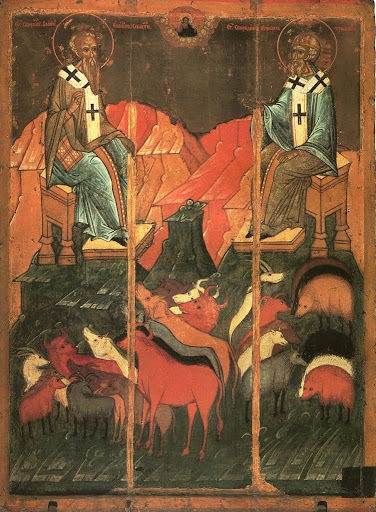
\includegraphics[width=0.80\linewidth]{chast-colebanie-osnov/tur/spiro.jpg}
\end{center}


   День святого Спиридона это 12 декабря по старому, 25 по новому стилю. Зимнее солнцестояние, выпадало на этот день в 16-17 веках, тогда же святой Спиридон и прослыл в народе Солнцеворотом. А вот 25 декабря по старому стилю, или 7 января по новому, солнцестояние было около 2000 лет назад, и к тому давнему солнцестояню церковь приурочила рождение Христа. Отмечу, что нигде в Библии не сказано, в какой день, месяц и год родился Иисус.

   Ни в григорианском, ни в юлианском календарях солнцестояние сейчас уже не выпадает на Рождество, ни католическое, ни православное.

   У скандинавов известен праздник зимнего солнцеворота Йоль, так похожий именем на нашу ёлку. Йоль означает полено, которое сжигали на протяжении 12 дней, и затем собирали уголь для обрядов. Подобным образом на Украине ставили дома под Рождество диду\'х – первый или последний сноп сена, перевязанный и украшенный, а потом сжигали его уже под Крещение.

   Вероятно, начало зимних празднований у язычников-славян сперва соответствовало  солнцестоянию. С усовершенствованием же календаря – мы не знаем какого – празднования могли быть уже привязаны к календарному дню и при несовершенстве календаря стали смещаться прочь от солнцестояния, как мы видим происходит с Рождеством в юлианском и григорианских календарях.

   Разумеется, обычай, или празднование Коляды на Рождество – языческий, но что означает это слово? В украинском названии
Рождества – «Різдво» сохранилось буквальное обозначение действия – забой скота. «Різдво» – от «різати», а «Коляда» – от «колоть». Известно, что в селах под Коляду, под Рождество колят, его не спросив, кабана к праздничному столу. Отсюда и слово «колдовство» – это искаженное «колядовство», ибо колдовство подразумевало и жертву.

   Коляда. Заколоть. Теперь напомню отрывок из жития святого Власия, что когда его заключили в темницу, то вдова, которой ранее помог Власий,

\begin{quotation}
заколола своего поросенка, который невредимым получился из зубов волка, сварила голову и ноги, положила на блюдо, сюда же она добавил еще семян, земных плодов и огородных овощей. Спрятав все это в корзинку, и зажегши свечу, она принесла эту корзинку святому в темницу. Припав к ногам мученика, стала умолять его, чтбы он взял эту пищу и вкусил ея. Воздав хвалу богу, святый вкусил принесенной пищи, затем, благословив вдову, он сказал ей:

 – Женщина, таким образом совершай каждый год мою память – тогда ничто из нужного в доме твоем не оскудеет, если же кто другой уподобится тебе и будет совершать мою память, тот получит в изобилии дары Божии и благословение господа пребудет на нем во все время его жизни.
\end{quotation}

   Церковь не предписывает подобного обряда – он просочился в житие святого Власа, чтобы оправдать существующий обычай, связанный со скотьим богом Волосом. Но ведь, скажете вы, Коляда, когда закалывают несчастных свиней, не выпадает на день святого Власа.

    Зато не лишним будет напомнить, что традиционным блюдом для Васильева вечера – Щедрого вечера – был приготовленный поросенок.

   Одному мне кажется, что и Влас, и Василий созвучны с Волосом?

   Смотрите – да вы это уже и сами заметили по песне-авсеньке – есть целая череда зимних праздников с обрядами, связанными с домашними животными, и эти праздники приурочены то к святым с именами, созвучными с Волосом, то к святому, чье имя само переводится как пастух, а то к святому, коего называют Овчаром.

   Полагаю, весь этот промежуток времени – от солнцестояния по нынешнее Крещение – был отведен на празднества, связанные с Волосом, скотьим богом.

   Церковь сосредоточила в сии дни поминовения созвучных по имени святых – причем святые эти приобрели свойства или обряды, связанные с домашними животными.

   В случае с Василием будто нет прямого свойства покровительства скоту, зато мы видим, что на Васильев вечер ходят ряженый козой и котом люди, а на стол подают убитого поросенка – то, что предписывал святой Власий – не Василий – в своем житии. Наконец, под праздник Василия кличут Авсеня-Усеня, в песнях уже непосредственно связанного с домашними животными.

    Животноводческая тема перенеслась и на святых с именами не созвучными с Волосом – Вукол отдельный случай, он сам по себе в переводе пастух, а вот Онисим стал Овчаром.

   Теперь вернемся ко крещению Руси Владимиром! Предположим, идол Волоса стоял тогда там же, где и Перун – около нынешней верхней станции фуникулера! Именно предположим, потому что источники молчат о местоположении идола.

   Вот Владимир низвергает идола Волоса с горы. Ставит там церковь Василия – созвучного Волосу. Но идола Волоса ставить там снова уже негде.

   Тогда, предположу, капище переносят в местность, что прослыло как урочище Турово – подальше от христианского духовенства, притом на Подол, вниз, поближе к народу. Водоток Турец же так назвался от того, что по нему потом из году в год, продолжая справлять обряд, сходный с похоронами русалок, тащили Тура – Волоса – в Иорданское озеро, а из него в Почайну и оттуда в Днепр.

   А по Днепру куда? Об этом – в последней главе книги.
